\chapter{Tổng quan dự án và Mô hình kinh doanh}
\label{chap:phan1_phan2}

% ==================== PHẦN 1: TỔNG QUAN & SWOT ====================
\section{Tổng quan dự án và Phân tích thị trường}

\subsection{Giới thiệu tổng quan về dự án}
Dự án tập trung vào việc xây dựng một Nền tảng Đọc Truyện Tranh Số Bản Quyền. Ý tưởng kinh doanh cốt lõi là tạo ra một hệ sinh thái khép kín kết nối trực tiếp độc giả, tác giả và đội ngũ quản trị. Mục tiêu của dự án là giải quyết vấn nạn truyện lậu đang gây thiệt hại lớn cho các tác giả, đồng thời nắm bắt cơ hội lấp đầy khoảng trống của thị trường bằng một nền tảng được nội địa hóa sâu hơn. Đối tượng khách hàng mục tiêu là thế hệ Gen Z, những người đã quen với việc chi tiêu cho giải trí số và thường xuyên sử dụng ví điện tử. Phạm vi dự án bao gồm việc phân phối truyện tranh kỹ thuật số tối ưu cho trải nghiệm trên thiết bị di động (đặc biệt là webtoon) và triển khai mô hình thanh toán vi mô (micro-transaction) thuận tiện.

\subsection{Phân tích thị trường}
\begin{itemize}
    \item \textbf{Kích thước và xu hướng thị trường:} Thị trường truyện tranh số toàn cầu dự kiến đạt 7-9 tỷ USD vào năm 2024 và dự báo tăng trưởng thần tốc lên mức 14.4 tỷ USD vào năm 2034. Tại thị trường nội địa, quy mô thương mại điện tử Việt Nam năm 2024 chạm mốc 25-32 tỷ USD với tốc độ tăng trưởng 27\%. Các xu hướng nổi bật bao gồm sự bùng nổ của định dạng truyện dọc (webtoon) trên toàn cầu và xu hướng "shoppertainment" (kết hợp mua sắm và giải trí).
    \item \textbf{Đặc điểm nhân khẩu học:} Việt Nam có tỷ lệ thâm nhập internet lên tới 78\% và có hơn 50\% dân số ở độ tuổi dưới 40. Với tập khách hàng này, đặc biệt là khách hàng thuộc thế hệ Gen Z, sẵn sàng trả tiền cho nội dung số chất lượng qua các nền tảng như Spotify hay Netflix.
    \item \textbf{Hành vi và Phân khúc:} Thông qua các khảo sát về \textit{Nhân khẩu học}, \textit{Thể loại truyện yêu thích}, \textit{Nền tảng đọc truyện} và \textit{Khả năng sẵn sàng chi trả}, nhóm thu được kết quả như sau:

    \begin{itemize}
        \item Có tới 96.4\% người dùng mục tiêu có đọc truyện online, tập trung chủ yếu ở nhóm 19-22 tuổi (48.2\%) và 23-25 tuổi (23.2\%).
        \item Thể loại truyện mà đa số khách hàng được khảo sát yêu thích nhất là Hành động/Phiêu lưu (69.6\%) và Tình cảm/Lãng mạn (53.6\%).
        \item Dù có tới 62.5\% khách hàng được khảo sát đang sử dụng web lậu, nhưng có tới 70.3\% lượng người dùng sẵn sàng trả tiền cho nội dung bản quyền nếu mức giá hợp lý.
        \item Mức giá lý tưởng (sweet spot) đối với người dùng là 1.000-5.000 đ/chương hoặc các gói Premium dao động từ 20.000-50.000 đ/tháng.
    \end{itemize}
\end{itemize}

\subsection{Nỗi đau của khách hàng (Pain Points)}
\textbf{Đối với Độc giả:}
\begin{itemize}
    \item Khoảng 94.4\% người dùng đang gặp ít nhất một vấn đề về trải nghiệm (UX) khi sử dụng các nền tảng hiện tại.
    \item Giao diện (UI) của các ứng dụng đọc truyện phổ biến đang bị đánh giá khá thấp (chỉ đạt điểm trung bình 3.2/5).
    \item Quảng cáo xuất hiện quá nhiều, làm gián đoạn mạch đọc (vấn đề lớn nhất - chiếm 90.7\% phản hồi).
    \item Tốc độ tải hình ảnh chậm chạp, hay giật lag trên thiết bị di động (79.6\%).
    \item Ứng dụng không lưu tiến độ đọc giữa các phiên, gây phiền toái cho người dùng (61.1\%).
    \item Việc đột ngột yêu cầu trả tiền (paywall) ở ngay những chương quan trọng khiến 59.3\% người dùng bực bội và bỏ đọc.
    \item Thiếu các kênh tương tác với tác giả, dù có tới 57.4\% người đọc rất quan tâm đến việc kết nối cộng đồng này.
\end{itemize}

\textbf{Đối với Tác giả:}
\begin{itemize}
    \item Bị mất doanh thu và không thể kiểm soát việc phân phối tác phẩm do vấn nạn sao chép, đăng lậu truyện.
    \item Mô hình kiếm tiền (monetization) bị hạn chế, chỉ phụ thuộc vào quảng cáo hoặc gói đăng ký (subscription) mà thiếu công cụ thanh toán vi mô.
    \item Hoàn toàn thiếu hụt bảng điều khiển (dashboard) phân tích để nắm bắt hành vi đọc truyện của độc giả.
    \item Ít có cơ hội tương tác trực tiếp với người đọc do nền tảng thiếu không gian blog, bình luận hay Q\&A.
    \item Thủ tục tham gia nền tảng (onboarding) thủ công, chi phí cao và quy trình tải truyện phức tạp tạo rào cản lớn.
\end{itemize}

\subsection{Phân tích SWOT}
\begin{table}[H]
    \centering
    \renewcommand{\arraystretch}{1.5}
    \begin{tabular}{|>{\raggedright\arraybackslash}p{0.45\textwidth}|>{\raggedright\arraybackslash}p{0.45\textwidth}|}
        \hline
        \multicolumn{1}{|c|}{\textbf{Điểm mạnh (Strengths)}} & \multicolumn{1}{c|}{\textbf{Điểm yếu (Weaknesses)}} \\
        \hline
        \vspace{-0.3cm}
        \begin{itemize}
            \item Tích hợp hệ thống chống sao chép bảo vệ bản quyền tác giả.
            \item Có hệ sinh thái khép kín: người đọc, tác giả, quản trị viên.
            \item UI ưu tiên chế độ tối, tốc độ tải ảnh cực nhanh nhờ MinIO + CDN.
            \item Chấp nhận thanh toán vi mô linh hoạt qua các ví điện tử.
            \item Phát triển tính năng cộng đồng mạnh mẽ (blog, Q\&A, bình luận).
        \end{itemize}
        & 
        \vspace{-0.3cm}
        \begin{itemize}
            \item Đòi hỏi chi phí hạ tầng ban đầu (server, CDN) lớn.
            \item Kho truyện giai đoạn đầu còn khiêm tốn so với các web lậu.
            \item Ngân sách marketing eo hẹp, mức độ nhận diện thương hiệu chưa cao.
            \item Sự phát triển phụ thuộc vào việc thu hút được tác giả sáng tạo.
            \item Đội ngũ kỹ thuật còn nhỏ gọn.
        \end{itemize} \\
        \hline
        \multicolumn{1}{|c|}{\textbf{Cơ hội (Opportunities)}} & \multicolumn{1}{c|}{\textbf{Thách thức (Threats)}} \\
        \hline
        \vspace{-0.3cm}
        \begin{itemize}
            \item Thị trường truyện tranh số toàn cầu dự báo sẽ tăng gấp 3 lần đến năm 2034.
            \item 59.3\% độc giả quen dùng ví điện tử, sẵn sàng thanh toán vi mô.
            \item Ý thức tôn trọng bản quyền số tại Việt Nam đang có xu hướng cải thiện.
            \item Gen Z đã có thói quen trả tiền cho các dịch vụ nội dung số (như Spotify).
            \item Cộng đồng tác giả chuyên nghiệp ngày càng mở rộng.
        \end{itemize}
        & 
        \vspace{-0.3cm}
        \begin{itemize}
            \item 90\% độc giả hiện đã quen với việc tiêu thụ nội dung lậu miễn phí.
            \item Cạnh tranh khốc liệt từ các ông lớn quốc tế (Webtoon, Tapas, Manga+).
            \item Khó khăn trong việc thay đổi thói quen cố hữu của người dùng.
            \item Đối diện với rủi ro bảo mật hệ thống và tấn công mạng (DDoS).
            \item Tính pháp lý đối với nội dung số còn nhiều điểm chưa rõ ràng.
        \end{itemize} \\
        \hline
    \end{tabular}
    \caption{Ma trận phân tích SWOT của nền tảng}
    \label{tab:swot}
\end{table}

\textbf{Phân tích chiến lược:} Khảo sát cho thấy nguyên nhân chính khiến người dùng tìm đến web lậu không hẳn do thiếu ý thức bản quyền, mà bởi thị trường chưa có mô hình thanh toán vi mô (micro-payment) đủ hấp dẫn. Dự án có thể tận dụng \textbf{Điểm mạnh} về hạ tầng tải nhanh và hệ thống thanh toán ví điện tử để khai thác tối đa \textbf{Cơ hội} từ tệp Gen Z sẵn sàng chi trả, qua đó giải quyết trực tiếp các \textbf{Thách thức} về thói quen dùng đồ miễn phí. Đồng thời, các tính năng tương tác độc quyền giữa tác giả và độc giả sẽ là lợi thế cạnh tranh quan trọng bù đắp cho \textbf{Điểm yếu} về số lượng nội dung ban đầu, giúp tạo ra tỷ lệ giữ chân khách hàng (retention) cao hơn so với các đối thủ trên thị trường.

% ==================== PHẦN 2: MÔ HÌNH KINH DOANH ====================
\section{Mô hình kinh doanh}

\subsection{Business Model Canvas (BMC)}
\begin{figure}[htbp]
    \centering
    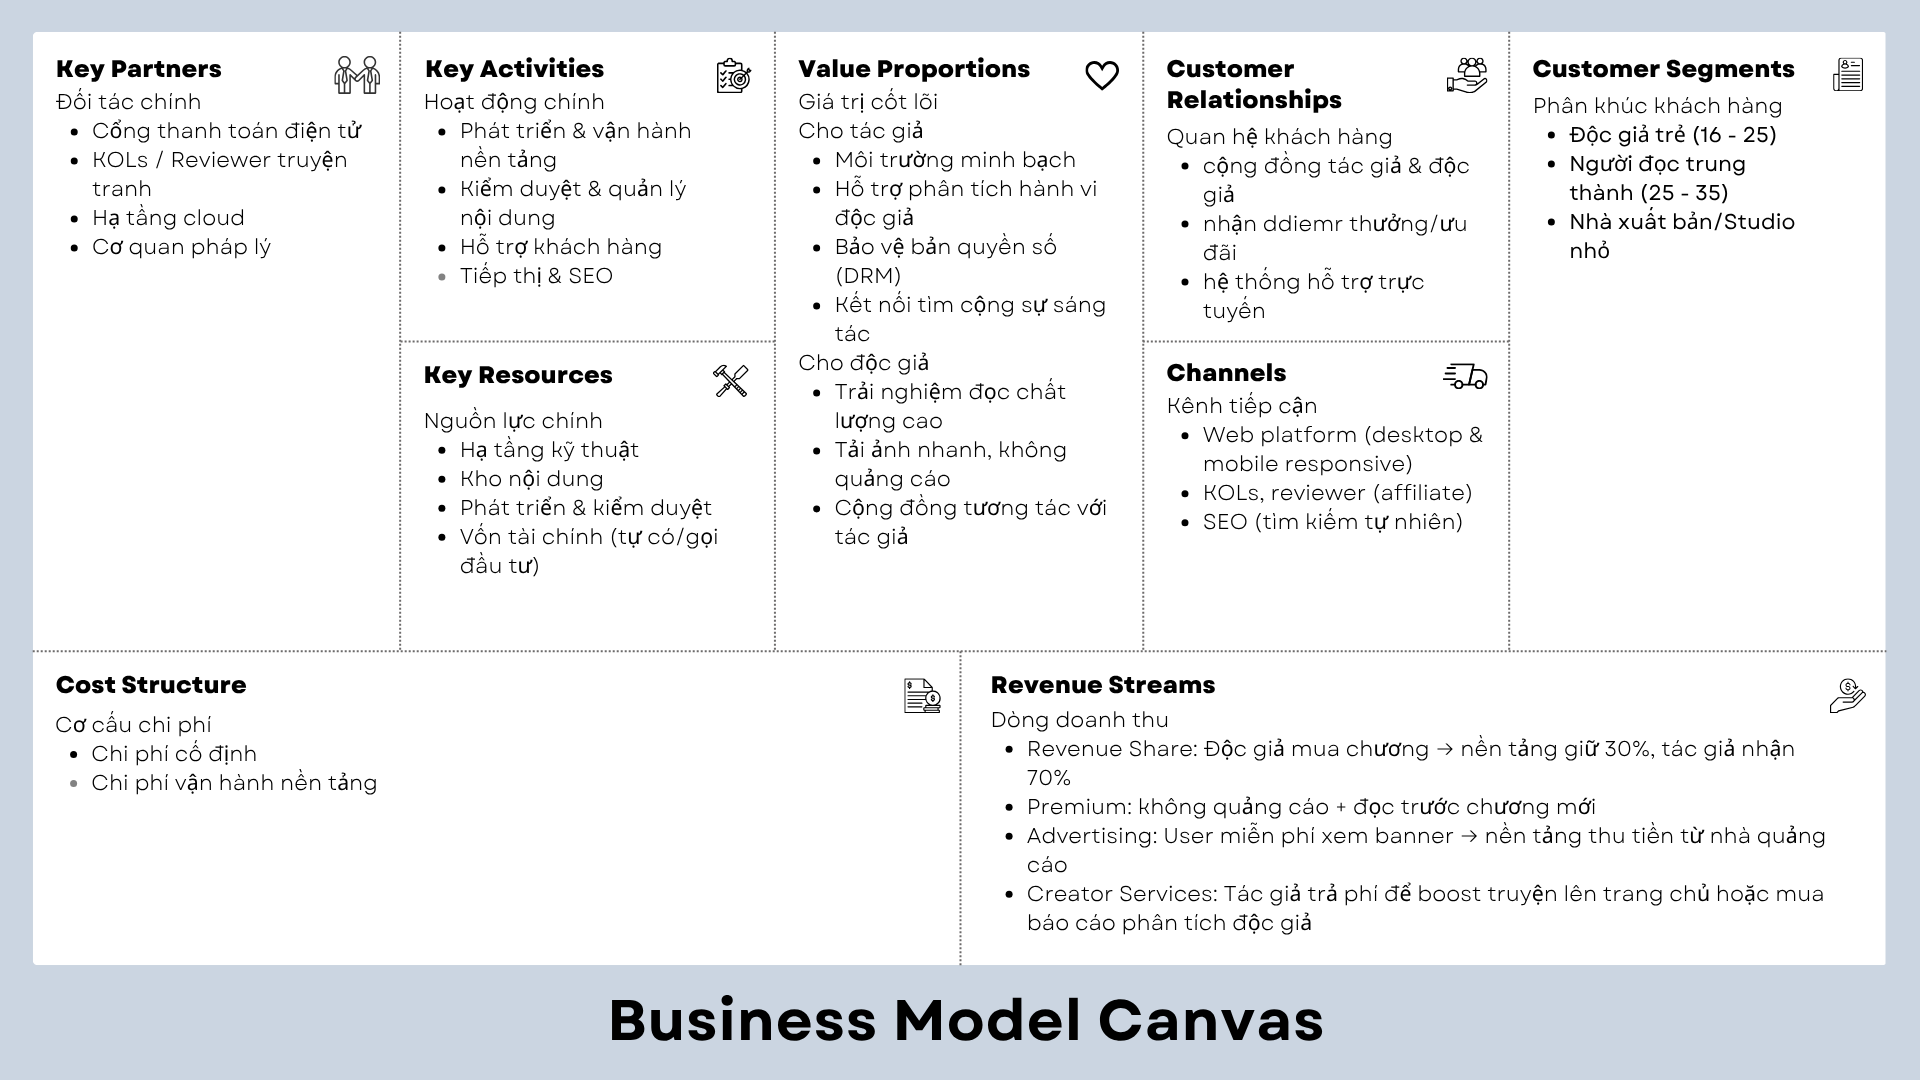
\includegraphics[width=\textwidth]{images/Diagram/BMC.png}
    \caption{Mô hình Business Model Canvas của nền tảng}
    \label{fig:bmc}
\end{figure}

Mô hình kinh doanh của dự án (chi tiết ở Hình \ref{fig:bmc}) được xây dựng theo khung Business Model Canvas (BMC) gồm 9 thành tố, xoay quanh việc tạo ra một hệ sinh thái kết nối hai nhóm đối tượng chính: Tác giả sáng tạo nội dung và Độc giả tiêu thụ nội dung. Việc vận hành trơn tru giữa nền tảng công nghệ, luồng phân phối nội dung và hệ thống thanh toán vi mô (micro-transaction) là xương sống của mô hình này.

\subsection{Phân tích chi tiết các thành phần chính}

\subsubsection{Value Proposition (Giá trị cốt lõi)}
\textbf{Dành cho Tác giả:}
\begin{itemize}
    \item \textbf{Hoạt động minh bạch:} Phân chia doanh thu rõ ràng, cung cấp dashboard ghi nhận doanh thu và dữ liệu theo thời gian thực.
    \item \textbf{Bảo vệ bản quyền:} Tích hợp cơ chế ngăn chặn sao chép trái phép (DRM) và báo cáo vi phạm tự động.
    \item \textbf{Công cụ sáng tạo \& Onboarding:} Quy trình đăng ký đơn giản, hỗ trợ kỹ thuật/pháp lý, cho phép upload chapter dễ dàng, lên lịch đăng chương và thông báo đến người theo dõi.
    \item \textbf{Kết nối \& Cộng đồng:} Hỗ trợ tương tác trực tiếp với người đọc qua Q\&A, bình luận, và tìm kiếm cộng sự sáng tác.
\end{itemize}

\textbf{Dành cho Độc giả:}
\begin{itemize}
    \item \textbf{Trải nghiệm đọc tối ưu:} Tải ảnh cực nhanh, không gián đoạn (hỗ trợ gói không quảng cáo), giao diện full-screen, tự động lưu tiến độ và đồng bộ đa thiết bị.
    \item \textbf{Thanh toán linh hoạt:} Áp dụng mô hình thanh toán vi mô lẻ từng chương (1.000 - 5.000 VNĐ/chương) hoặc gói Premium (20.000 - 50.000 VNĐ/tháng) tích hợp tiện lợi qua các Ví điện tử.
    \item \textbf{Khám phá thông minh:} Hệ thống tìm kiếm nâng cao theo thể loại, tác giả và bộ lọc gợi ý thông minh dựa trên lịch sử đọc cá nhân.
    \item \textbf{Tương tác cộng đồng:} Tham gia bình luận theo từng chương, nhận thông báo chương mới tức thì.
\end{itemize}

\subsubsection{Customer Segments (Phân khúc khách hàng)}
\begin{itemize}
    \item \textbf{Độc giả trẻ (16-25 tuổi):} Nhóm người dùng có thời gian đọc nhiều, thói quen đọc online mạnh mẽ, đòi hỏi cao về trải nghiệm UX/UI tối ưu.
    \item \textbf{Người đọc trung thành (25-35 tuổi):} Nhóm có thu nhập ổn định, sẵn sàng chi trả và ưu tiên nội dung chất lượng cao hơn là việc tiết kiệm.
    \item \textbf{Tác giả / Creator nội địa:} Những người sáng tạo nội dung truyện tranh cần nền tảng để xuất bản, bảo vệ bản quyền và kiếm tiền.
    \item \textbf{Nhà xuất bản / Studio nhỏ:} Đơn vị muốn phân phối số hóa các tác phẩm đã có bản quyền và chia sẻ doanh thu theo thỏa thuận hợp tác.
\end{itemize}

\subsubsection{Revenue Streams (Dòng doanh thu)}
\begin{itemize}
    \item \textbf{Revenue Share (Nguồn thu cốt lõi):} Độc giả mua chương lẻ, nền tảng giữ 30\%, tác giả nhận 70\%. Với tác giả ký hợp đồng độc quyền, tỷ lệ ưu đãi có thể lên tới 80\% (tác giả) - 20\% (nền tảng).
    \item \textbf{Premium Subscription ($\sim$30\% tổng thu):} Gói hội viên khoảng 49.000 VNĐ/tháng. Quyền lợi: Không quảng cáo, đọc trước chương mới 3-7 ngày, cấp hạn mức chương miễn phí.
    \item \textbf{Advertising ($\sim$10\% tổng thu):} Cung cấp không gian quảng cáo (banner cuối chương, tối đa 1 banner/chương) hướng đến nhóm người dùng đọc miễn phí.
    \item \textbf{Creator Services ($\sim$5\% tổng thu):} Các dịch vụ giá trị gia tăng thu phí từ tác giả như đẩy truyện (boost) lên trang chủ, hoặc cung cấp báo cáo phân tích hành vi độc giả nâng cao.
\end{itemize}

\subsubsection{Cost Structure (Cơ cấu chi phí)}
\textbf{Chi phí cố định:}
Đây là các khoản chi phí nền tảng cần thiết để thiết lập và duy trì bộ máy hoạt động độc lập với doanh thu hiện tại.
\begin{itemize}
    \item \textbf{Chi phí phát triển sản phẩm:} Ngân sách đầu tư ban đầu cho việc thiết kế UI/UX, lập trình, kiểm thử và xây dựng hoàn thiện hệ thống ứng dụng (Web/PWA, Backend, API).
    \item \textbf{Lương cho Nhân sự:} Quỹ lương chi trả định kỳ cho đội ngũ vận hành hệ thống, bao gồm đội ngũ kỹ thuật (Developer), ban quản trị nội dung (Admin), chăm sóc khách hàng và đội ngũ pháp lý.
    \item \textbf{Chi phí Hạ tầng mạng cơ bản:} Các khoản phí cố định để duy trì hệ thống máy chủ cốt lõi (server), cơ sở dữ liệu quan hệ (PostgreSQL) và các chứng chỉ bảo mật nền tảng.
    \item \textbf{Chi phí Pháp lý:} Phí đăng ký bản quyền thương hiệu, tư vấn luật Sở hữu trí tuệ, soạn thảo hợp đồng hợp tác với tác giả và chi phí giải quyết các tranh chấp pháp lý.
\end{itemize}

\textbf{Chi phí Vận hành (Chi phí biến đổi):}
Đây là các khoản phí biến đổi theo mức độ quy mô, lượng người dùng và hiệu quả kinh doanh của nền tảng.
\begin{itemize}
    \item \textbf{Chi phí Băng thông và Lưu trữ:} Phí duy trì Cloud Storage (MinIO) và mạng phân phối nội dung (CDN). Chi phí này tăng tỷ lệ thuận với khối lượng ảnh truyện được tải lên bởi tác giả và lưu lượng truy cập đọc truyện của người dùng.
    \item \textbf{Chi phí chia sẻ doanh thu:} Khoản chi phí cốt lõi chiếm tỷ trọng lớn khi phân phối lại doanh thu cho Tác giả (thường từ 70\% đến 80\%) cho mỗi lượt mua chương trả phí hoặc doanh thu từ gói Premium.
    \item \textbf{Chi phí Marketing:} Ngân sách dành cho các chiến dịch quảng cáo, duy trì mạng lưới đối tác liên kết (Affiliate), trả phí cho KOLs/Reviewer và các hoạt động SEO để thu hút độc giả mới.
\end{itemize}

\subsubsection{Key Resources (Nguồn lực chính):}
\begin{itemize}
    \item \textit{Công nghệ \& Hạ tầng:} Hệ thống CDN tải ảnh nhanh, nền tảng mã nguồn, kiến trúc server, và công nghệ bảo mật.
    \item \textit{Con người:} Đội ngũ phát triển (Dev), đội ngũ quản lý cộng đồng/nội dung, và đội ngũ pháp lý.
    \item \textit{Mạng lưới \& Tài chính:} Kho nội dung ban đầu, tệp tác giả tự do, vốn tự có và vốn gọi từ các nhà đầu tư.
\end{itemize}

\subsubsection{Key Activities (Hoạt động chính):}
\begin{itemize}
    \item \textit{Phát triển \& Duy trì nền tảng:} Xây dựng hệ thống web/PWA, quy trình CI/CD, giám sát (monitor) và cập nhật tính năng liên tục.
    \item \textit{Quản lý Nội dung \& Bản quyền:} Kiểm duyệt bộ truyện tác giả gửi lên, quét và xử lý các vi phạm bản quyền.
    \item \textit{Vận hành luồng tài chính:} Xử lý thanh toán an toàn và phân phối chia sẻ doanh thu minh bạch cho đối tác.
\end{itemize}

\subsubsection{Key Partners (Đối tác chính):}
\begin{itemize}
    \item Cổng thanh toán điện tử / Ví điện tử (MoMo, ZaloPay, VietQR).
    \item Nhà cung cấp dịch vụ hạ tầng Cloud (AWS, MinIO).
    \item Mạng lưới KOLs / Manga Reviewer.
    \item Các cơ quan pháp lý và bảo vệ bản quyền.
\end{itemize}

\subsubsection{Customer Relationships (Quan hệ khách hàng):}
\begin{itemize}
    \item Nuôi dưỡng cộng đồng kết nối trực tiếp giữa Tác giả và Độc giả.
    \item Triển khai hệ thống điểm thưởng, ưu đãi cho khách hàng thân thiết và người dùng gói Premium.
    \item Duy trì dịch vụ hỗ trợ trực tuyến đa kênh: Chatbot, FAQ, và Live Chat.
\end{itemize}

\subsubsection{Channels (Kênh tiếp cận \& phân phối):}
\begin{itemize}
    \item \textit{Nền tảng trực tiếp:} Web platform responsive, PWA (Progressive Web App).
    \item \textit{Cộng đồng \& Affiliate:} Hợp tác với KOLs, Reviewer (chia hoa hồng 5-10\% cho mỗi lượt giới thiệu).
    \item \textit{Content Marketing \& SEO:} Xây dựng blog review, tối ưu hóa long-tail keyword (ví dụ: "đọc [tên truyện] bản quyền online"), áp dụng schema markup.
    \item \textit{Email \& Push Notification:} Gửi Bản tin (newsletter) hàng tuần, thông báo (push) chương mới, và chiến dịch Re-engagement nhắc nhở người dùng quay lại đọc truyện.
\end{itemize}

\subsection{Logic vận hành và sự liên kết giữa các khối}
Mô hình hoạt động theo nguyên lý "Nền tảng đa phía" (Multi-sided Platform), trong đó \textbf{Giá trị cốt lõi} được hình thành từ sự cộng sinh giữa Nguồn nội dung (Tác giả) và Lượng truy cập (Độc giả).

\begin{itemize}
    \item \textbf{Bước 1 (Thu hút nguồn lực):} Nền tảng sử dụng \textbf{Key Resources} (Hạ tầng mạnh, công cụ quản lý) và \textbf{Key Activities} (Onboarding dễ dàng, cam kết bảo vệ bản quyền) để thuyết phục Tác giả tham gia. Nguồn nội dung chất lượng chính là thỏi nam châm hút người dùng.
    \item \textbf{Bước 2 (Tiếp cận \& Phân phối):} Qua các \textbf{Channels} (SEO, KOLs Affiliate, PWA), nền tảng mang nội dung tiếp cận đúng \textbf{Customer Segments} (Gen Z và người trưởng thành yêu truyện). 
    \item \textbf{Bước 3 (Giao dịch \& Khóa chặt khách hàng):} Nhờ \textbf{Key Partners} (Ví điện tử) hỗ trợ các vi giao dịch mượt mà, kết hợp với \textbf{Customer Relationships} (hệ thống cộng đồng, điểm thưởng, thông báo Push), nền tảng biến người đọc miễn phí thành người dùng trả phí.
    \item \textbf{Bước 4 (Tạo dòng tiền):} Dòng tiền đổ về qua các \textbf{Revenue Streams} (bán chương lẻ, gói Premium, dịch vụ Tác giả, và Quảng cáo) sẽ bù đắp lại cho \textbf{Cost Structure} (chi phí CDN, server, duy trì đội ngũ). Dòng tiền này tiếp tục được chia sẻ lại cho Tác giả (Revenue Share 70-80\%), tạo động lực để họ sản xuất nội dung mới, tạo thành một bánh đà tăng trưởng (flywheel) khép kín và bền vững.
\end{itemize}
